\documentclass[11pt]{article}
\usepackage[margin=0.82in]{geometry}
\usepackage{amsmath,amssymb,amsthm,mathtools}
\usepackage{graphicx,booktabs,array,enumitem,microtype}
\usepackage[dvipsnames]{xcolor}
\usepackage[colorlinks=true,linkcolor=NavyBlue,citecolor=NavyBlue,urlcolor=NavyBlue]{hyperref}

\newtheorem{theorem}{Theorem}
\newtheorem{proposition}[theorem]{Proposition}
\newtheorem{lemma}[theorem]{Lemma}
\newtheorem{corollary}[theorem]{Corollary}
\newcommand{\Bmeet}{\mathbin{\curlywedge_{\!B}}}
\newcommand{\one}{\mathbf 1}

\title{General Boolean Spectral Maxima and the Missing\\Type-I and Type-III Extreme Values}
\author{Autonomous solution packet for arXiv:2003.05382, Problem 2.17}
\date{11 August 2026}

\begin{document}
\maketitle

\begin{abstract}
We answer both clauses of Problem 2.17.  For any two probability laws on
$\mathbb R$, the canonical Boolean product gives Boolean-independent
selfadjoint operators with those laws whose spectral maximum has an explicit
distribution.  At negative thresholds its CDF is an endpoint test; at
nonnegative thresholds it is $FG/(F+G-FG)$.  This defines an associative
max-operation on all real laws.  The same model, followed by ordinary affine
normalization of the maximum, realizes three Boolean extreme-value limits:
Dagum (type II), logistic (type I), and a bounded reciprocal-power family
(type III).
\end{abstract}

\section{The question and the answer}

Problem 2.17 of Ueda asks for operator models realizing the maximum of
Boolean-independent general selfadjoint operators and for Boolean extreme
values other than the positive Dagum family \cite{Ueda2020}.  The exact source
text is reproduced below.

\begin{center}
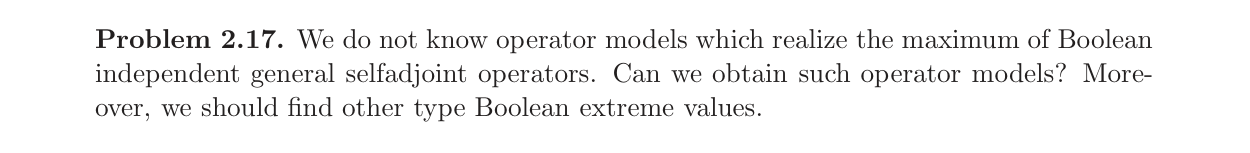
\includegraphics[width=0.94\textwidth]{figures/problem_2_17_crop.png}
\end{center}

For $p,q\in[0,1]$, put
\begin{equation}\label{eq:B}
 p\Bmeet q=\begin{cases}
 \dfrac{pq}{p+q-pq},&p+q>0,\\[4pt]
 0,&p=q=0.
 \end{cases}
\end{equation}
Thus $(p\Bmeet q)^{-1}-1=(p^{-1}-1)+(q^{-1}-1)$ when
$p,q>0$.  This is the scalar Boolean projection operation of
Vargas--Voiculescu \cite[Lemma 3.1]{VV2018}.

\begin{theorem}[arbitrary-selfadjoint Boolean maximum]\label{thm:model}
Let $\mu_1,\mu_2$ be arbitrary probability measures on $\mathbb R$.  There
are Boolean-independent, possibly unbounded, selfadjoint operators
$\widehat X_1,\widehat X_2$ with respective vector-state laws
$\mu_1,\mu_2$.  If $F_i(t)=\mu_i(({-\infty},t])$, then their spectral maximum
has CDF
\begin{equation}\label{eq:diamond}
F_{\widehat X_1\vee\widehat X_2}(t)=
\begin{cases}
1,&t<0\ \text{and}\ F_1(t)=F_2(t)=1,\\
0,&t<0\ \text{and at least one of }F_1(t),F_2(t)\text{ is }<1,\\
F_1(t)\Bmeet F_2(t),&t\geq0.
\end{cases}
\end{equation}
The construction is canonical from the two marginal multiplication models.
Formula \eqref{eq:diamond} defines an associative operation on all real
distribution functions and is realized simultaneously for every finite
number of Boolean-independent copies.
\end{theorem}

The distinguished point $0$ is not an artificial choice: it is the zero
operator on the orthogonal complement introduced by the nonunital Boolean
product.  Positivity in the earlier theory merely ensures that only the third
line of \eqref{eq:diamond} is visible.

\begin{theorem}[three Boolean extreme-value types]\label{thm:types}
For every $\alpha>0$, normalized spectral maxima of positive,
Boolean-independent selfadjoint operators in the model of
Theorem~\ref{thm:model} have each of the following nondegenerate limits:
\begin{align*}
B_{\mathrm{II},\alpha}(x)
 &=\begin{cases}(1+x^{-\alpha})^{-1},&x>0,\\0,&x\leq0,
 \end{cases}\\[2pt]
B_{\mathrm I}(x)&=(1+e^{-x})^{-1},\qquad x\in\mathbb R,\\[2pt]
B_{\mathrm{III},\alpha}(x)
 &=\begin{cases}(1+(-x)^\alpha)^{-1},&x\leq0,\\1,&x>0.
 \end{cases}
\end{align*}
The first is the known Dagum/type-II law.  The logistic law $B_{\mathrm I}$
and the bounded law $B_{\mathrm{III},\alpha}$ give the requested type-I and
type-III Boolean extreme values.
\end{theorem}

\section{Proof intuition}

The Boolean product Hilbert space contains the two centered marginal spaces
and one shared vacuum line.  Each variable acts as its original multiplication
operator on its own centered space plus the vacuum, and as zero on the other
centered space.  Consequently its lower spectral projection has two different
forms.  Below zero the foreign zero-space is excluded; at and above zero it is
included.  Intersecting the two lower spectral subspaces therefore gives an
endpoint test below zero and the familiar Boolean projection formula above
zero.

For extreme values, the scalar homeomorphism
\[
 \chi(u)=\begin{cases}e^{1-u^{-1}},&u>0,\\0,&u=0,
 \end{cases}
 \qquad \chi^{-1}(v)=\begin{cases}(1-\log v)^{-1},&v>0,\\0,&v=0,
 \end{cases}
\]
turns $\Bmeet$ into multiplication.  Thus positive Boolean maxima are the
pullback under $\chi$ of classical maxima.  Allowing the usual centering only
\emph{after} taking the operator maximum avoids the unit problem noted in the
earlier Boolean theory.  Pulling back the three classical limits gives the
three formulas in Theorem~\ref{thm:types}.

\section{The canonical operator model}

For $i=1,2$, let
\[
 H_i=L^2(\mathbb R,\mu_i),\qquad \xi_i=\one,
 \qquad X_i=M_x,
 \]
where $M_x$ is the maximal multiplication operator.  Put
$K_i=H_i\ominus\mathbb C\xi_i$ and
\[
 H=\mathbb C\Omega\oplus K_1\oplus K_2.
\]
Let $V_i:H_i\to H$ be the isometry that sends $\xi_i$ to $\Omega$ and is the
identity from $K_i$ to its displayed summand.  Define
\begin{equation}\label{eq:copies}
 \widehat X_1=(V_1X_1V_1^*)\oplus 0_{K_2},\qquad
 \widehat X_2=(V_2X_2V_2^*)\oplus 0_{K_1},
\end{equation}
with the evident direct-sum domains.  These are selfadjoint even when the
marginal multiplication operators are unbounded, and
$\langle f(\widehat X_i)\Omega,\Omega\rangle=\int f\,d\mu_i$.

The nonunital operator families $V_i\mathcal B(H_i)V_i^*$ are Boolean
independent for the vacuum state.  Indeed, if adjacent indices alternate,
then $V_i^*V_j=|\xi_i\rangle\langle\xi_j|$ for $i\ne j$, so direct
multiplication gives
\[
 \langle A_1\cdots A_m\Omega,\Omega\rangle
 =\prod_{k=1}^m\langle A_k\Omega,\Omega\rangle.
\]
This is precisely Boolean factorization.  It also proves that
\eqref{eq:copies} depends only on the two marginal models.

We record the projection computation used below.

\begin{lemma}[Boolean projection join]\label{lem:proj}
Let $R,S$ be Boolean-independent projections and set
$p=\varphi(I-R)$, $q=\varphi(I-S)$.  Then
\[
 \varphi\bigl(I-(R\vee S)\bigr)=p\Bmeet q.
\]
\end{lemma}

\begin{proof}
This is \cite[Lemma 3.1]{VV2018}; a short derivation makes the packet
self-contained.  The Cauchy and Boolean cumulant transforms of $R$ are
\[
G_R(z)=\frac pz+\frac{1-p}{z-1}=\frac{z-p}{z(z-1)},
\qquad K_R(z)=z-G_R(z)^{-1}=\frac{z(1-p)}{z-p},
\]
and similarly for $S$.  Boolean additivity gives
$K_{R+S}=K_R+K_S$.  Since
$\ker(R+S)=\ker R\cap\ker S=\operatorname{ran}(I-(R\vee S))$, its vacuum
mass is the atom of $R+S$ at zero.  Hence
\[
\varphi(I-(R\vee S))
=\lim_{z\to0}zG_{R+S}(z)
=\frac1{p^{-1}+q^{-1}-1}=p\Bmeet q,
\]
with the endpoint cases obtained by continuity.
\end{proof}

\begin{proof}[Proof of Theorem~\ref{thm:model}]
Let $A_i(t)=E_{X_i}(({-\infty},t])$ and $P_i(t)=
E_{\widehat X_i}(({-\infty},t])$.  Functional calculus in the direct sum
\eqref{eq:copies} gives
\begin{equation}\label{eq:spectral-split}
P_1(t)=\begin{cases}V_1A_1(t)V_1^*,&t<0,\\
V_1A_1(t)V_1^*+P_{K_2},&t\geq0,
\end{cases}
\end{equation}
and the symmetric formula for $P_2(t)$.

Suppose first that $t<0$.  The ranges of $P_1(t)$ and $P_2(t)$ lie in
$\mathbb C\Omega\oplus K_1$ and $\mathbb C\Omega\oplus K_2$, whose
intersection is $\mathbb C\Omega$.  Their intersection contains $\Omega$ if
and only if $A_i(t)\xi_i=\xi_i$ for both $i$.  Since $A_i(t)$ is a
projection, this is equivalent to
$\langle A_i(t)\xi_i,\xi_i\rangle=F_i(t)=1$.  Thus the first two lines of
\eqref{eq:diamond} follow.

Now let $t\geq0$.  Formula \eqref{eq:spectral-split} yields
\[
 I-P_i(t)=V_i(I-A_i(t))V_i^*=:R_i(t).
\]
The two $R_i(t)$ are Boolean-independent projections and
$\varphi(I-R_i(t))=F_i(t)$.  Because the lower spectral projection of the
spectral maximum is $P_1(t)\wedge P_2(t)$, Lemma~\ref{lem:proj} gives
\[
F_{\widehat X_1\vee\widehat X_2}(t)
=\varphi(P_1(t)\wedge P_2(t))
=\varphi(I-(R_1(t)\vee R_2(t)))
=F_1(t)\Bmeet F_2(t).
\]

The right side of \eqref{eq:diamond} is increasing and right-continuous; at
zero its left limit can be one only when both $F_i(0)=1$.  It therefore is a
CDF.  Below zero its scalar operation is ``one iff every input is one,''
which is associative.  At nonnegative thresholds, associativity follows from
the additivity of $u^{-1}-1$.  For finitely many marginal spaces, replace
$H$ by $\mathbb C\Omega\oplus\bigoplus_iK_i$.  The same proof, or the atom at
zero of the sum of all complementary projections, gives the corresponding
finite-fold formula.
\end{proof}

For a CDF $F$, write $F^{\diamond n}$ for the CDF of the maximum of $n$
canonical Boolean copies.  The preceding proof gives, for $n\geq2$,
\begin{equation}\label{eq:nfold}
F^{\diamond n}(t)=
\begin{cases}
\one_{\{F(t)=1\}},&t<0,\\[2pt]
\dfrac{F(t)}{n-(n-1)F(t)},&t\geq0.
\end{cases}
\end{equation}

\section{Extreme-value transfer and the two new types}

The identity
\begin{equation}\label{eq:chi}
 \chi(p\Bmeet q)=\chi(p)\chi(q)
\end{equation}
is immediate from \eqref{eq:B}.  Consequently, if $K$ is a CDF supported on
$[0,\infty)$ and $F=\chi^{-1}\circ K$, then, whenever $y\geq0$,
\begin{equation}\label{eq:transfer}
 \chi\bigl(F^{\diamond n}(y)\bigr)=K(y)^n.
\end{equation}
Thus every classical normalization whose evaluation points are eventually
nonnegative transfers to the Boolean model.  We now give explicit parents,
so no appeal to a general domain-of-attraction theorem is needed.

\paragraph{Type II (Fr\'echet $\longrightarrow$ Dagum).}
Let
\[
K_{0,\mathrm{II}}(y)=
\begin{cases}0,&y<1,\\1-y^{-\alpha},&y\geq1,
\end{cases}
\qquad F_{0,\mathrm{II}}=\chi^{-1}\circ K_{0,\mathrm{II}}.
\]
If $M_n$ is the spectral maximum of $n$ canonical Boolean copies with law
$F_{0,\mathrm{II}}$, then, for $x>0$,
\[
\chi\!\left(F_{M_n/n^{1/\alpha}}(x)\right)
=\left(1-\frac{x^{-\alpha}}n\right)^n
\longrightarrow e^{-x^{-\alpha}}.
\]
For $x\leq0$ the limit is zero.  Applying $\chi^{-1}$ gives
$B_{\mathrm{II},\alpha}$.

\paragraph{Type I (Gumbel $\longrightarrow$ logistic).}
Take the exponential CDF
\[
K_{0,\mathrm I}(y)=\begin{cases}0,&y<0,\\1-e^{-y},&y\geq0,
\end{cases}
\qquad F_{0,\mathrm I}=\chi^{-1}\circ K_{0,\mathrm I}.
\]
For every fixed $x$, the point $x+\log n$ is nonnegative for all large $n$,
and \eqref{eq:transfer} gives
\[
\chi\!\left(F_{M_n-\log n}(x)\right)
=\left(1-\frac{e^{-x}}n\right)^n
\longrightarrow e^{-e^{-x}}.
\]
Therefore $M_n-\log n$ converges in distribution to
\[
\chi^{-1}(e^{-e^{-x}})=\frac1{1+e^{-x}},
\]
the logistic CDF.

\paragraph{Type III (reverse Weibull $\longrightarrow$ bounded reciprocal power).}
Let
\[
K_{0,\mathrm{III}}(y)=
\begin{cases}
0,&y<0,\\
1-(1-y)^\alpha,&0\leq y\leq1,\\
1,&y>1,
\end{cases}
\qquad F_{0,\mathrm{III}}=\chi^{-1}\circ K_{0,\mathrm{III}}.
\]
For $x\leq0$ and all large $n$,
\[
\chi\!\left(F_{n^{1/\alpha}(M_n-1)}(x)\right)
=\left(1-\frac{(-x)^\alpha}{n}\right)^n
\longrightarrow e^{-(-x)^\alpha};
\]
for $x>0$ the CDF is already one.  Applying $\chi^{-1}$ gives
$B_{\mathrm{III},\alpha}$.  This proves Theorem~\ref{thm:types}.

\section{Why centering is legitimate}

Earlier treatments avoided shifts of the \emph{inputs}, because adjoining a
common scalar identity to Boolean-independent nonunital algebras destroys the
naive Boolean product picture \cite[Section 2]{VV2018}.  Here no input is
shifted.  We first form the spectral maximum $M_n$ inside the canonical
Boolean product and only then apply the ordinary selfadjoint affine map
$a^{-1}(M_n-bI)$.  For $a>0$ its CDF is exactly
$F_{M_n}(ax+b)$, which is all that was used above.  Hence the type-I and
type-III constructions do not assume Boolean independence of translated
copies and do not encounter the unit obstruction.

\section{Scope and verification}

Theorem~\ref{thm:model} is an existence model determined by the marginals; it
does not assert that the spectral maximum has the same law in every possible
realization of Boolean independence.  This is precisely the operator-model
existence requested in Problem 2.17.  The formulas include atoms, unbounded
marginal multiplication operators, and all threshold edge cases.

The accompanying verifier checks \eqref{eq:chi}, the type-I and type-III
limits, and finite-dimensional canonical models with mixed-sign and purely
negative spectra.  In those models it constructs the lower spectral
projections, computes their range intersection numerically, and compares the
vacuum mass to \eqref{eq:diamond}.

\begin{thebibliography}{9}
\bibitem{Ueda2020}
Y.~Ueda,
\emph{Max-convolution semigroups and extreme values in limit theorems for the
free multiplicative convolution}, arXiv:2003.05382 (2020), Problem 2.17.

\bibitem{VV2018}
J.~G.~Vargas and D.~V.~Voiculescu,
\emph{Boolean Extremes and Dagum Distributions}, arXiv:1711.06227 (2018),
especially Sections 2--4 and Lemmas 3.1--3.3.
\end{thebibliography}

\end{document}

